

\tikzset{every picture/.style={line width=0.75pt}} %set default line width to 0.75pt        

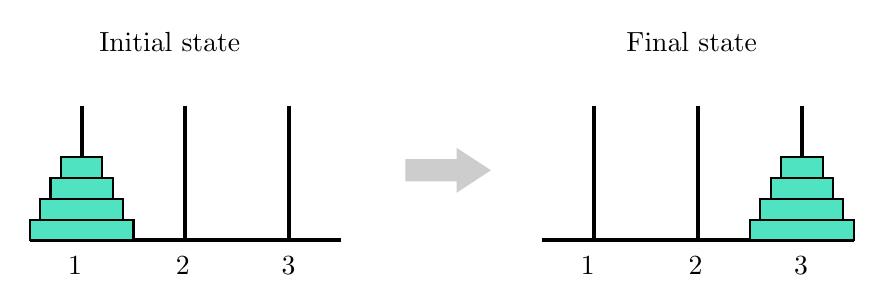
\begin{tikzpicture}[x=0.75pt,y=0.75pt,yscale=-1,xscale=1]
%uncomment if require: \path (0,265); %set diagram left start at 0, and has height of 265

%Straight Lines [id:da47303320704215723] 
\draw [line width=1.5]    (203,153) -- (203,88) ;
%Straight Lines [id:da2596274943436139] 
\draw [line width=1.5]    (253,153) -- (253,88) ;
%Straight Lines [id:da6158417047874292] 
\draw [line width=1.5]    (153,153) -- (153,88) ;
%Straight Lines [id:da5552650208095853] 
\draw [line width=1.5]    (128,153) -- (278,153) ;
%Shape: Rectangle [id:dp7871559520719595] 
\draw  [fill={rgb, 255:red, 80; green, 227; blue, 194 }  ,fill opacity=1 ] (143,113) -- (163,113) -- (163,123) -- (143,123) -- cycle ;
%Shape: Rectangle [id:dp16971724332757798] 
\draw  [fill={rgb, 255:red, 80; green, 227; blue, 194 }  ,fill opacity=1 ] (138,123) -- (168,123) -- (168,133) -- (138,133) -- cycle ;
%Shape: Rectangle [id:dp543708016051085] 
\draw  [fill={rgb, 255:red, 80; green, 227; blue, 194 }  ,fill opacity=1 ] (133,133) -- (173,133) -- (173,143) -- (133,143) -- cycle ;
%Shape: Rectangle [id:dp0244026959370931] 
\draw  [fill={rgb, 255:red, 80; green, 227; blue, 194 }  ,fill opacity=1 ] (128,143) -- (178,143) -- (178,153) -- (128,153) -- cycle ;

%Straight Lines [id:da7221147779404855] 
\draw [line width=1.5]    (450,153) -- (450,88) ;
%Straight Lines [id:da7874597275294666] 
\draw [line width=1.5]    (500,153) -- (500,88) ;
%Straight Lines [id:da4225603478965123] 
\draw [line width=1.5]    (400,153) -- (400,88) ;
%Straight Lines [id:da3778502666400989] 
\draw [line width=1.5]    (375,153) -- (525,153) ;
%Shape: Rectangle [id:dp10843492640608887] 
\draw  [fill={rgb, 255:red, 80; green, 227; blue, 194 }  ,fill opacity=1 ] (490,113) -- (510,113) -- (510,123) -- (490,123) -- cycle ;
%Shape: Rectangle [id:dp31674744674602295] 
\draw  [fill={rgb, 255:red, 80; green, 227; blue, 194 }  ,fill opacity=1 ] (485,123) -- (515,123) -- (515,133) -- (485,133) -- cycle ;
%Shape: Rectangle [id:dp2873092905375003] 
\draw  [fill={rgb, 255:red, 80; green, 227; blue, 194 }  ,fill opacity=1 ] (480,133) -- (520,133) -- (520,143) -- (480,143) -- cycle ;
%Shape: Rectangle [id:dp6845419069966949] 
\draw  [fill={rgb, 255:red, 80; green, 227; blue, 194 }  ,fill opacity=1 ] (475,143) -- (525,143) -- (525,153) -- (475,153) -- cycle ;

%Right Arrow [id:dp18178145046985472] 
\draw  [draw opacity=0][fill={rgb, 255:red, 155; green, 155; blue, 155 }  ,fill opacity=0.5 ] (309,113.81) -- (333.71,113.81) -- (333.71,108.41) -- (350.18,119.2) -- (333.71,130) -- (333.71,124.6) -- (309,124.6) -- cycle ;

% Text Node
\draw (391.99,159.4) node [anchor=north west][inner sep=0.75pt]    {$1$};
% Text Node
\draw (443.91,159.4) node [anchor=north west][inner sep=0.75pt]    {$2$};
% Text Node
\draw (494.83,159.4) node [anchor=north west][inner sep=0.75pt]    {$3$};
% Text Node
\draw (144.99,159.4) node [anchor=north west][inner sep=0.75pt]    {$1$};
% Text Node
\draw (196.91,159.4) node [anchor=north west][inner sep=0.75pt]    {$2$};
% Text Node
\draw (247.83,159.4) node [anchor=north west][inner sep=0.75pt]    {$3$};
% Text Node
\draw (160,51) node [anchor=north west][inner sep=0.75pt]   [align=left] {Initial state };
% Text Node
\draw (414,51) node [anchor=north west][inner sep=0.75pt]   [align=left] {Final state };


\end{tikzpicture}